\documentclass[12pt]{article}

\usepackage[utf8]{inputenc}
\usepackage{amsthm,amssymb,amsmath,dsfont,mathrsfs,nicefrac,wasysym,listings}
\usepackage{tikz}
\usepackage{enumitem}


\usetikzlibrary{shapes,arrows}


\let\stdsection\section
\renewcommand\section{\newpage\stdsection}

\renewcommand{\arraystretch}{1.1}

\lstloadlanguages{Haskell}
\lstnewenvironment{haskell}
    {\lstset{}%
      \csname lst@SetFirstLabel\endcsname}
    {\csname lst@SaveFirstLabel\endcsname}
    \lstset{
      basicstyle=\small\ttfamily,
      escapeinside={/+}{+/},
      flexiblecolumns=false,
      xleftmargin=0.05\textwidth,
      basewidth={0.5em,0.45em},
      literate={+}{{$+$}}1
               {/}{{$/$}}1
               {*}{{$*$}}1
               {=}{{$=$}}1
               {>}{{$>$}}1
               {<}{{$<$}}1
               {\\}{{$\lambda$}}1
               {++}{{$+\!\!\!+$}}1
               {::}{{$:\!\!\!:$}}1
               {\\\\}{{\char`\\\char`\\}}1
               {->}{{$\rightarrow$}}2
               {>=}{{$\geq$}}2
               {<-}{{$\leftarrow$}}2
               {<=}{{$\leq$}}2
               {=>}{{$\Rightarrow$}}2
               {/=}{{$\neq$}}2
               {.}{{$\circ$}}2
               {<<}{{$\ll$}}2
               {>>}{{$\gg$}}2
               {>>=}{{$\gg\!=$}}2
               {>=>}{{$>\!=\!>$}}2
               {|}{{$\mid$}}1
               {undefined}{{$\bot$}}1
               {`elem`}{{$\in$}}1
    }

\title{Title of my paper}
\author{Thomas Dybdahl Ahle}
\date{March 9, 2013}

\begin{document}
\maketitle

\begin{abstract}
Your abstract goes here...

Érica is super hot

‘a brief description of what you did; no more than a page.’
The abstract provides a summary of the project report. It may contain some or all of the following moves, 
often, but not always, in the following order. Only use one or two sentences for each move. Keep the 
language and sentence structure simple. The reader should be able to read the abstract and obtain the 
necessary information quickly and efficiently.
Move 1:  Background to the project
Move 2: Purpose of the project
Move 3: Problem tackled
Move 4: Work carried out
Move 5: Results 
Move 6: Conclusions or implications
Move 7: Achievements of the project

\end{abstract}

\tableofcontents


\section{Introduction}
5 pagish Donkey example to follow through. There are many reasons why it is interesting to represent information in a logical language. You can do things such as unification, resolution, and question answering.

Move 1 Background 
Possible Steps 1. Why the area is important
2. Giving background information
3. Reviewing previous research
Move 2 Indicating a Problem or Need
Move 3 Presenting the Project
Possible Steps 1. Purposes, aims, objectives
2. Work carried out
3. Justification or importance of the project
4. Outline of the structure of the report

In this paper we won't do anything about animal violence

% Define block styles
\tikzstyle{decision} = [diamond, draw, fill=blue!20,
    text width=4.5em, text badly centered, node distance=2.5cm, inner sep=0pt]
\tikzstyle{block} = [rectangle, draw, fill=blue!20,
    text width=5em, text centered, rounded corners, minimum height=4em]
\tikzstyle{line} = [draw, -latex']
    
\begin{tikzpicture}[node distance = 3cm, auto]
    % Place nodes
    \node [block] (nl) {Natural Language};
    \node [block, right of=nl] (dr) {Dependency Representation};
    \node [block, right of=dr] (monad) {Enhanced DPL Representation};
    \node [block, right of=monad] (dpl) {Dynamic Propositional Logic};
    \node [block, right of=dpl] (prop) {First Order Logic};
    % Draw edges
    \path [line] (nl) -- (dr);
    \path [line] (dr) -- (monad);
    \path [line] (monad) -- (dpl);
    \path [line] [dotted] (dpl) -- (prop);
\end{tikzpicture}

% It is not possible
It is clear that not all sentences can be unambigiously translated from natural language to logic. A sentence like 	
\begin{quotation}
A farmer beats a donkey
\end{quotation}
Might be translated as 
\begin{equation}
\exists x ( farmer(x) \wedge \exists y ( donkey(y) \wedge beats(x,y)))
\end{equation}
Indicating that ``a farmer'' refers to some specific individual. Or we can might see it as a general rule, and translate it as
\begin{equation}
\forall x ( farmer(x) \rightarrow \exists y ( donkey(y) \wedge beats(x,y)))
\end{equation}
Indicating that every farmer has some donkey he beats. Or we could even read it as
\begin{equation}
\exists y ( donkey(y) \wedge \forall x ( farmer(x) \rightarrow beats(x,y)))
\end{equation}
Indicating that the poor donkey is common between all farmers.
% This seams wrong to me

Additionally, the indefinite article `a' is normally understood as an existential quantifier

Week and strong readings, check this out \cite{kanazawa1994weak}

In this paper we will not try to solve the above problem. (Though it could be interesting to generate multiple possibilities and perhaps use context to filter out the correct one). Instead we will try to show how some old method for doing this conversion can be enhanced with some new tools

\begin{equation}
\forall x . farmer(x) \rightarrow (\forall y . donkey(y) \wedge owns(x,y) \rightarrow beats(x,y))
\end{equation}

This one has problems with scope
\begin{equation}
\forall x (farmer(x) \wedge \exists y (donkey(y) \wedge owns(x,y) \rightarrow beats(x,y)))
\end{equation}

Moving the scope doesn't solve it, since now if there are two donkeys and he only owns one of them, the sentence will be true nomatter if he beats them or not. Also if he owns say a donkey and a horse, the left part of the implication would be vacously true and hence the beats part wouldn't matter.
\begin{equation}
\forall x \exists y (farmer(x) \wedge donkey(y) \wedge owns(x,y) \rightarrow beats(x,y))
\end{equation}


If a farmer owns a donkey he beats it
\begin{equation}
\forall x . farmer(x) \rightarrow (\forall y . donkey(y) \wedge owns(x,y) \rightarrow beats(x,y))
\end{equation}

There are a lot of problems with this representation
\begin{itemize}
  \item It is not compositional. 
  dfdf
  \item It doesn't very well follow the order of the original sentence
  \item It is just not very easy to get right
\end{itemize}

More stuff from wikipedia:

Unfortunately, this translation leads to a serious problem of inconsistency. Indefinites must sometimes be interpreted as existential quantifiers, and other times as universal quantifiers, without any apparent regularity

More questions:

Should those three have the same meaning?
[1a]  Jane likes a painting.
[1b]  It is not the case that Jane doesn't like a painting.
[1c]  Jane likes a painting and either it is raining or it isn't.


\section{Formal Stuff}
10 pagish

This subsection's content...

Background should introduce any information that is necessary for the examiner to understand your project. 
The information here is generally more specific than the background given in the Introduction.
Requirements gives the program requirements. These chapters prepare the ground for the Design chapter.
That is: What do we need to handle to be able to solve this problem

In particular, anaphora resolution is part of DRT, but in dynamic semantic systems anaphora resolution is assumed to be performed by a separate component of the theory

\subsection{DPL}
Dynamic semantics: http://plato.stanford.edu/entries/dynamic-semantics/

growth of information in time
Inspired by programming language
not philosofically, states can be anything. I don't want to get into that
isomorphic with normal logic (visser siger generalization/projection)
doen't promise to be a perfect dual of natural language, but it's closer, and has been rewarding
Dynamic semantics aims to model meaning and interpretation. You can do that without answering broader philosophical questions
takes the meaning of concepts for given
dynamic assignment language, discourse representation theory, file change, update semantics, 
Jan van Eijck, Hans Kamp, Veltman, Groenendijk

compoitionality. A man comes in. He sees a dog. He smiles.

Vi har brug for en logik, der ikke behøver at vide alting fra starten

direct translation not possible
`He saw the man with the telescope'
and even if we understand the syntax
`The students all attended one class'
has at least two meanings.
interpretation of discourse is influenced and guided by the common ground that exists between speaker and hearer

relation between sets of assignments
$\{\overline{PQR}, \overline{PQ}R, \overline{P}Q\overline{R}, \overline{P}QR, P\overline{QR}, P\overline{Q}R, PQ\overline{R}, PQR\}$

example

real world example

hvad med sudoku. I started er alle assignments mulige. Nae.. Men. hm

something about more information, less models
the interpretation of false

Something about kleiski combinator?

the thing about quantifiers
how they would work in a programming language
$\exists x; A$
$\exists x; x = 4$ hvis $x=4$ skal virke og reducere mængden af modeller, så må exists gøre dem alle sammen mulige

A man comes in. En fri variabel vi ikke ved noget om.
A man comes in. It's Thomas..

we take as DPL-meanings binary relations between assignments

later we will use an isomorphism and take them as functions from assignments to sets of assignments.

\begin{equation}
\phi ::= \bot \mid \top \mid \pi \mid \epsilon \mid \phi \cdot \phi \mid \lnot(\phi)
\end{equation}
\begin{equation}
\alpha [\bot] \beta :\equiv False
\end{equation}
\begin{equation}
\alpha [\top] \beta :\equiv \alpha = \beta
\end{equation}
\begin{equation}
\alpha[P(x_0, ..., xn-1)]\beta :\equiv \alpha = \beta and (\alpha x0, ..., \alpha x n-1 ) \in I(P)
\end{equation}

\subsection{Connection with first order logic}

normal logik kan også laves om til dpl. Nemt, bare brug not.not til at scope E.

An alternative way of defining the semantics

Shows that we aren't doing anything `odd' or `fancy'

shows sound and complete wrt.

Preconditions
weakest phi sa <phi> pi <T> is still true

Like hoare stuff

inspired Dynamic assignment language \cite{eijck1992dynamic}
Jan van Eijck 
Fer-Jan de Vries 

like using a stack

$\alpha \models \langle\psi\rangle\phi$ iff there is an assignment $\beta$ with $\alpha[\psi]\beta$, and $\beta \models \phi$

Definition of true and false $\alpha\models\phi :\leftrightarrow \exists\beta(alpha\phi\beta)$.

%{

%Det her skal med for at vi kan forsvare ligningerne

%α[⊥]β :⇔ 0 ≠ 0.
%α[⊤]β :⇔ α = β.
%α[P(x0, …, xn−1)]β :⇔ α = β and ⟨αx0, …, αxn−1 ⟩ ∈ I(P), 
%where P is a predicate symbol of Σ with arity n.
%α[∃v]β :⇔ α[v]β, where α[v]β iff αw = βw, for all variables w ≢ v.
%α[φ · ψ]β :⇔ ∃γ  α[φ]γ[ψ]β.
%α[~(φ)]β :⇔ α = β and ∀γ  ¬ α[φ]γ.
%

Det giver ikke mening at skrive $\not\models[\psi]$ da typen af $[\psi]$ er en relation. Eller hvad?

\begin{align}
\alpha[\psi_1\cdot\psi_2]\beta &:\leftrightarrow \exists\gamma (\alpha[\psi_1]\gamma \wedge \gamma[\psi_2]\beta) \label{sem_and} \\
\alpha[\psi_1\cup\psi_2]\beta &:\leftrightarrow \alpha[\psi_1]\beta \vee \alpha[\psi_2]\beta \label{sem_or} \\
\alpha[P(x_1,\dots,x_n)]\beta &:\leftrightarrow \alpha = \beta \wedge P(\alpha_{x_1},\dots,\alpha_{x_n}) \label{sem_pred} \\
\alpha[\neg\psi]\beta &:\leftrightarrow \alpha = \beta \wedge \alpha\not\models[\psi] \label{sem_neg}\\
\alpha[\exists x]\beta &:\leftrightarrow \forall\omega (\omega \neq x \rightarrow \alpha_{\omega} = \beta_{\omega}) \label{sem_exists} \\
\intertext{Using these we can derive the following:}
\alpha[\bot]\beta &\leftrightarrow \alpha = \beta \wedge \bot \nonumber\\
                  &\leftrightarrow \bot \label{sem_bot}\\
\alpha[\top]\beta &\leftrightarrow \alpha = \beta \wedge \top \nonumber\\
                  &\leftrightarrow \alpha = \beta \label{sem_top}\\
\intertext{Taking $\psi_1\rightarrow\psi_2$ to mean $\neg(\psi_1\wedge\neg\psi_2)$ we also get the following neat equation, originally by Groenendijk and Stokhof\cite{groenendijk1991dynamic}:}
\alpha[\psi_1\rightarrow\psi_2]\beta
 &:\leftrightarrow \alpha[\neg(\psi_1\wedge\neg\psi_2)]\beta \nonumber\\
 &\leftrightarrow \alpha = \beta \wedge \alpha\not\models[\psi_1\wedge\neg\psi_2] \nonumber\\
 &\leftrightarrow \alpha = \beta \wedge \neg\exists\gamma(\alpha[\psi_1\wedge\neg\psi_2]\gamma) \nonumber\\
 &\leftrightarrow \alpha = \beta \wedge \neg\exists\gamma(\exists\delta(\alpha[\psi_1]\delta\wedge\delta[\neg\psi_2]\gamma)) \nonumber\\
 &\leftrightarrow \alpha = \beta \wedge \neg\exists\gamma(\exists\delta(\alpha[\psi_1]\delta\wedge\delta=\gamma\wedge\delta\not\models[\psi_2])) \nonumber\\
 &\leftrightarrow \alpha = \beta \wedge \forall\gamma(\forall\delta(\delta=\gamma\rightarrow(\alpha[\psi_1]\delta\rightarrow\delta\models[\psi_2]))) \nonumber\\
 &\leftrightarrow \alpha = \beta \wedge \forall\gamma(\alpha[\psi_1]\gamma\rightarrow\gamma\models[\psi_2]) \label{sem_impl}
\end{align}

Hence we can read implication as a the filter, that if you can get `through' $\psi_1$ then you must also be able to get through $\psi_2$. Also notice that $\gamma$ doesn't have to equal $\alpha$. Hence variables introduced in $\psi_1$ can bind variables in $\psi_2$. This will show to be extreamly important in the treatment of donkey sentences later.

Talking about binding, also notice that our union or `or' construct is a bit special. $\psi_1$ and $\psi_2$ cannot bind variables in each other, but in $(\psi_1\cup\psi_2)\cdot\psi_3$ they can both bind variables in $\psi_3$. This is going to introduce a lot of weird situations later. An alternative definition of `or': $\neg(\neg\psi_1\cdot\neg\psi_2)$ will also be considered.

For \eqref{sem_pred} $P$ is a predicate symbol of $\Sigma$ with arity n.

static negation. DOesn't allow new things. LIke a filter

some people have a closed/static or: $\neg(\neg\psi_1\wedge\neg\psi_2)$ \cite{groenendijk1991dynamic}

%Notice that \eqref{sem_bot} and \eqref{sem_top} are special cases of \eqref{sem_pred}.

We are going to introduce formuals that allow us to recursively convert any DRA formula into PL.

To smoothen the following proofs, we will introduce a special syntax `$\langle\psi\rangle\phi$' where $\psi$ is a DRA formula, $\phi$ is a PL formula and the whole thing is a PL formula. For some assignment $\alpha$, we define `$\alpha\models\langle\psi\rangle\phi$' to mean $\exists\beta(\alpha[\psi]\beta \wedge \beta\models\phi)$.

\begin{align}
\alpha\models\langle\exists x\rangle\phi
 & \leftrightarrow \exists\beta (\alpha[\exists x]\beta \wedge \beta\models\phi) \nonumber\\
 & \leftrightarrow \exists\beta (\forall\omega (\omega \neq x \rightarrow \alpha_{\omega} = \beta_{\omega}) \wedge \beta\models\phi) \nonumber\\
 & \leftrightarrow \exists\beta (\exists\nu (\forall\omega (\alpha[x:=\nu]_{\omega} = \beta_{\omega})) \wedge \beta\models\phi) \nonumber\\
 & \leftrightarrow \exists\beta (\exists\nu (\alpha[x:=\nu] = \beta) \wedge \beta\models\phi) \nonumber\\
% & \leftrightarrow \exists\nu (\exists\beta (\alpha[x:=\nu] = \beta \wedge \beta\models\phi)) \nonumber\\
 & \leftrightarrow \exists\nu (\alpha[x:=\nu]\models\phi) \nonumber\\
 & \leftrightarrow \alpha\models\exists x (\phi) \label{conv_exists}\\\nonumber\\
%
\alpha\models\langle\psi_1\cdot\psi_2\rangle\phi
 & \leftrightarrow \exists\beta (\alpha[\psi_1\cdot\psi_2]\beta \wedge \beta\models\phi) \nonumber\\
 & \leftrightarrow \exists\beta(\exists\gamma (\alpha[\psi_1]\gamma \wedge \gamma[\psi_2]\beta) \wedge \beta\models\phi) \nonumber\\
 & \leftrightarrow \exists\gamma (\alpha[\psi_1]\gamma \wedge \exists\beta(\gamma[\psi_2]\beta \wedge \beta\models\phi)) \nonumber\\
 & \leftrightarrow \exists\gamma (\alpha[\psi_1]\gamma \wedge \gamma\models\langle\psi_2\rangle\phi) \nonumber\\
 & \leftrightarrow \alpha\models\langle\psi_1\rangle\langle\psi_2\rangle\phi \label{conv_and}\\\nonumber\\
%
\alpha\models\langle\psi_1 \cup \psi_2\rangle\phi
 & \leftrightarrow \exists\beta (\alpha[\psi_1 \cup \psi_2]\beta \wedge \beta\models\phi) \nonumber\\
 & \leftrightarrow \exists\beta ((\alpha[\psi_1]\beta \vee \alpha[\psi_2]\beta) \wedge \beta\models\phi) \nonumber\\
 & \leftrightarrow \exists\beta (\alpha[\psi_1]\beta \wedge \beta\models\phi) \vee \exists\beta (\alpha[\psi_2]\beta \wedge \beta\models\phi) \nonumber\\
 & \leftrightarrow (\alpha\models\langle\psi_1\rangle\phi) \vee (\alpha\models\langle\psi_2\rangle\phi) \nonumber\\
 & \leftrightarrow \alpha\models\langle\psi_1\rangle\phi \vee \langle\psi_2\rangle\phi \label{conv_or}\\\nonumber\\
%
\alpha\models\langle P(x_1,\dots,x_n)\rangle\phi
 & \leftrightarrow \exists\beta (\alpha[P(x_1,\dots,x_n)]\beta \wedge \beta\models\phi) \nonumber\\
 & \leftrightarrow \exists\beta (\alpha = \beta \wedge P(\alpha_{x_1},\dots,\alpha_{x_n}) \wedge \beta\models\phi) \nonumber\\
 & \leftrightarrow P(\alpha_{x_1},\dots,\alpha_{x_n}) \wedge \alpha\models\phi \nonumber\\
 & \leftrightarrow \alpha\models P(x_1,\dots,x_n) \wedge \phi \label{conv_pred}\\\nonumber\\
%
\alpha\models\langle\neg\psi\rangle\phi
 & \leftrightarrow \exists\beta (\alpha[\neg\psi]\beta \wedge \beta\models\phi) \nonumber\\
 & \leftrightarrow \exists\beta (\alpha=\beta \wedge \neg\exists\gamma(\alpha[\psi]\gamma) \wedge \beta\models\phi) \nonumber\\
 & \leftrightarrow \neg\exists\gamma(\alpha[\psi]\gamma) \wedge \alpha\models\phi \nonumber\\
 & \leftrightarrow \neg\exists\gamma(\alpha[\psi]\gamma \wedge \gamma\models\top) \wedge \alpha\models\phi \nonumber\\
 & \leftrightarrow \alpha\not\models\langle\psi\rangle\top \wedge \alpha\models\phi \nonumber\\
 & \leftrightarrow \alpha\models \neg\langle\psi\rangle\top \wedge \phi \label{conv_neg}
\end{align}

Notice that $\alpha\models\langle\bot\rangle\phi$ and $\alpha\models\langle\top\rangle\phi$ follow trivially from \eqref{conv_pred}.

\begin{haskell}
addDpl :: Prop -> [DPL] -> Prop
addDpl p [] = p
addDpl p (DF:ds) = F
addDpl p (DT:ds) = addDpl p ds
addDpl p ((DPredi f ks):ds) = addDpl (And (Predi f ks) p) ds
addDpl p ((DExists k):ds) = addDpl (Exist k p) ds
addDpl p ((DComp d1 d2):ds) = addDpl p (d2:d1:ds) -- backwards
addDpl p ((DNot d):ds) = addDpl (And (Not (addDpl T [d])) p) ds
addDpl p ((DImpl d1 d2):ds) = addDpl p ((DNot (DComp d1 (DNot d2))):ds)
addDpl p ((DOr d1 d2):ds) = addDpl (And (Or (addDpl T [d1]) (addDpl T [d2])) p) ds
\end{haskell}

\subsection{The problem with disjunction}


a farmer doesn't own a horse or a donkey

Ex.farmer(x) . ~(Ey.horse(y).owns(x,y) v Ey.donkey(y).owns(x,y))
Ex.farmer(x) . ~Ey.horse(y).owns(x,y) . ~Ey.donkey(y).owns(x,y)

a farmer beats a horse or a donkey

Ex.farmer(x).(Ey.horse(y) v Ez.donkey(z)).beats(x,y) = {Nothing, Ex.farmer(x).EyJust .horse(y).beats(x,y)}

Ex.farmer(x).~((Ey.horse(y) v Ez.donkey(z)).beats(x,y)) =
Ex.farmer(x).(~Ey.horse(y).~Ez.donkey(z) v ~beats(x,y)) = {Nothing, Ex.farmer(x).~Ey.horse(y).~Ez.donkey(z)}

Ex.farmer(x).~(tall(x) v blue(x)) = Ex.famer(x).~tall(x).~blue(x)

There is a farmer who maybe has a donkey. He beats it.
Ex.farmer(x).(Ey.donkey(y) v false).beats(x,y)
With union semantics for v this would be equal to
Ex.farmer(x).Ey.donkey(y).beats(x,y)
which is stupid.
Intead with sets of relations, this would be equal to
Ex.farmer(x).Ey.donkey(y).beats(x,y) v Ex.farmer(x).false.beats(x,y)
the right side being an error? no

If a farmer is not poor he owns a donkey. He beats it.
Ex.farmer(x).~poor(x) -> Ey.donkey(y).owns(x,y).beats(x,y)

A farmer is either poor or he owns a donkey. He beats it.
Ex.farmer(x).(poor(x) v Ey.donkey(y).owns(x,y)).beats(x,y) =

(Ex v false) . f(x)
(exist x `union` false) [] = [[("x",0)],[("x",1)],[("x",2)]
[Nothing, Just [[("x",0)],[("x",1)],[("x",2)]]]


(Ex v false) = [Just [[("x",0)],[("x",1)],[("x",2)], Just []]
not (Ex v false) =

not (Ex v f(x))
= ~Ex.~f(x)

A farmer owns a horse or a donkey
Ex.farmer(x).~(~(Ey.horse(y)).~(Ey.donkey(y))).owns(x,y)   this surely doesn't work


nothing survives out of a not (or impl) it's normal. Don't worry about it

Let's just say that if some of 
maybe not (bla v bla v bla v ERROR) should be ERROR
it could also be something more involved, like ERROR(bla v bla v bla v ERROR), but let's not do that
fmap

We can also try to define semantics using first order logic. This totally doesn't work and convert reasonable statements into mess. In particular it is hard to have or not being closed scopewise.

The difference between those two:

$addDpl p ((DOr d1 d2):ds) = addDpl (And (Or (addDpl T [d1]) (addDpl T [d2])) p) ds$

$addDpl p ((DOr d1 d2):ds) = Or (addDpl p (d1:ds)) (addDpl p (d2:ds))$


Fra Dynamic Montague Grammar:
This means that the extended dynamic semantics is also able to deal with a donkey
disjunction such as (49), and in such a way that it is equivalent with the donkey
conditional (50). It can further be noted that this notion of dynamic disjunction is
like dynamic implication in this respect that sentences which follow it, are in fact
conjoined with its second argument:
Fact 24 [either p or q] ; r = either p or [q ; r]
This is needed for a treatment of examples such as:
(54) Either there is no bathroom here, or it is in a funny place. In any case, it is
not on the ground floor.

Den ene giver mulighed for at binde fra a til b. Den anden giver mulighed for at begge dele binder res

\subsubsection{Weird disjunctive subjects}

problem wouldn't work in Spanish
A farmer or their donkey was arrested this morning.

\begin{equation}
Ex(farmer(x)) ^ Ey(donkey(y)) ^ (a-t-m(x) v a-t-m(y))
ExEy(farmer(x) ^ donkey(y) ^ owns(x,y) ^ (a-t-m(x) v a-t-m(y)))
Ex(farmer(x)) v Ey(donkey(y))
((Ex . farmer(x) . Es.s=x) v (Ey . donkey(y) . owns(x,y) . Es.s=y)) . a-t-m(s)
((Ex . farmer(x) . (Es.s=x v (Ey . donkey(y) . owns(x,y) . Es.s=y)) v (Ey . donkey(y) . owns(x,y) . Es.s=y)) . a-t-m(s)
\end{equation}

If a farmer is Spanish or a Japanese she beats her donkey
It is a donkey or a horse
You beat it or I do
Either a farmer or his donkey is happy

either = xor?

Vissers dynamic bracketing


\subsection{Errors}

Or should this be in implementation? Hard for me to say



\subsection{Monadic variants}
This might be what I call DRA underneath
In the previous subsection we saw that DPL allowed us to rewrite the donkey sentence as 

\begin{equation}
\exists x \cdot farmer(x) \cdot \exists y \cdot donkey(y) \cdot owns(x,y) \rightarrow beats(x,y)
\end{equation}

($\cdot$ binds stronger than $\rightarrow$)

But think about the slight modification to the sentence:
%
\begin{quotation}
A farmer owns a donkey, if he beats it
\end{quotation}
%
We would have to write that as
%
\begin{equation}
\exists x \cdot farmer(x) \cdot \exists y \cdot donkey(y) \cdot beats(x,y) \rightarrow owns(x,y)
\end{equation}
%
The problem here is that reorderings like this work against our sought property of linearity: of being able to add new information as we go. We cannot compose `A farmer owns a donkey' and `if he beats it' in a meaningful way.

To resque us from this problem Albert Visser suggests constructing a special e-monoid over the dynamic relational algebra. The idea is that we are going to simultaniously work on two `streams' of dpl, and switch easily between them with a special element $\Bowtie$.

Our sentence from above will then be expressible as
%
\begin{equation}
\Bowtie \cdot \exists x \cdot farmer(x) \cdot \exists y \cdot donkey(y) \cdot \Bowtie \cdot owns(x,y) \cdot \Bowtie \cdot beats(x,y)
\end{equation}
%
which can be written in `stream form' as
%
\begin{equation}
\begin{tabular}{|clll|}
    \hline
    $(-)$ & $\exists x \cdot farmer(x) \cdot \exists y \cdot donkey(y)$ & ~ & $beats(x,y)$ \\\hline
    $(+)$ & ~ & $owns(x,y)$ & ~ \\\hline
\end{tabular}
\end{equation}
%
The meaning of the above is $(-) \rightarrow (+)$

Should we have one more example here?

So how do we define this nifty $\Bowtie$? The trick is to move the entire dynamic relation algebra from before into an e-monoid that will help us keep track of some details.

If $\phi$ from before is the basic algebra, we specify the construction of our monoid $\Phi$ as follows.
%
\begin{flalign}
&\top := \langle \top, \top, + \rangle & \\
&\bot := \langle \top, \bot, + \rangle & \\
&\Bowtie := \langle \top, \top, - \rangle & \\
&\langle q_-, q_+, \alpha \rangle \cdot \langle r_-, r_+, \beta \rangle := \langle q_- \cdot r_{-\alpha}, q_+ \cdot r_{+\alpha}, \alpha\beta \rangle&
\end{flalign}
%
Notice how we keep the negative stream in the first position of the tuple, and the positive stream at the second position. The third position idicates to what stream we are currently writing. For example, if we are writing to the negative stream, and we apply an element that itself asks us to continue at its negative stream, we go back to the positive stream.

More examples on the utilities of the above monad can be found in Vissers paper.

An even more interesting element than $\Bowtie$ is $\triangle$. $\triangle$ is a scope modifier, and it allows us to write:
%
\begin{quote}
A farmer owns a donkey. He beats it.
\end{quote}
%
(that is just some single farmer and donkey) as
%
\begin{equation}
\triangle \cdot \exists x \cdot farmer(x) \cdot \triangle \cdot owns(x,y) \cdot \triangle \cdot \exists y \cdot donkey(y) \cdot \triangle \cdot beats(x,y)
\end{equation}
%
That is pretty close to the order of the natural language!

And combining the two monads we can do our original sentence as
%
\begin{quote}
If a farmer owns a donkey, he beats it
\end{quote}
%
as
\begin{equation}
\Bowtie \cdot \triangle \cdot \exists x \cdot farmer(x) \cdot \triangle \cdot owns(x,y) \cdot \triangle \cdot \exists y \cdot donkey(y) \cdot \triangle \cdot \Bowtie \cdot beats(x,y)
\end{equation}
%
In stream form, that is:
%
\begin{equation}
\begin{tabular}{|cllll|}
    \hline
    $(-,1)$ & $\exists x \cdot farmer(x)$ & ~ & ~ $ \exists y \cdot donkey(y)$ & ~ \\\hline
    $(-,0)$ & ~ & $owns(x,y)$ & ~ & ~ \\\hline
    $(+,1)$ & ~ & ~ & ~ & ~ \\\hline
    $(+,0)$ & ~ & ~ & ~ & $beats(x,y)$ \\\hline
\end{tabular}
\end{equation}
%
With the meaning being $(-,1) \cdot (-,0) \rightarrow (+,1) \cdot (+,0)$. Notice that the negative relations are again put on the left side of the implication, and the relations with larger scope value are put before those of lower value.

Notice $\Bowtie$ and $\triangle$ are commutative, since they work entirely on their own indicator. It's an interesting question to consider what sentences might require three or more levels of scoping, but those seam to be so rare that it doesn't now make much sense to clutter our algebra with an extra infinity of streams.

We define the monad as follows:
%
\begin{flalign}
&\top := \langle \top, \top, \top, \top, +, 0 \rangle & \\
&\bot := \langle \top, \top, \top, \bot, +, 0 \rangle & \\
&\Bowtie := \langle \top, \top, \top, \top -, 0 \rangle & \\
&\triangle := \langle \top, \top, \top, \top +, 1 \rangle & \\
&\langle q_{-,1}, q_{-,0}, q_{+,1}, q_{+,0}, \alpha, i \rangle \cdot \langle r_{-,1}, r_{-,0}, r_{+,1}, r_{+,0}, \beta, j \rangle := &\\
&\hspace{1cm}\langle q_{-,1} \cdot r_{-\alpha,1+i}, q_{-,0} \cdot r_{-\alpha,i}, q_{+,1} \cdot r_{\alpha,1+i}, q_{+,0} \cdot r_{\alpha,i}, \alpha\beta, i+j \rangle& \nonumber
\end{flalign}

In his paper Visser now goes on to define $\triangleleft$ and $\triangleright$ which work similarly to $\Bowtie$ except they work in different directions. 
%
\begin{equation}
\Bowtie \cdot \triangle \cdot \exists x \cdot farmer(x) \cdot \triangle \cdot owns(x,y) \cdot \triangle \cdot \exists y \cdot donkey(y) \cdot \triangle \cdot \triangleleft \cdot beats(x,y)
\end{equation}
%
This is quite interesting for certain centences containing `surprises', like
%
\begin{quotation}
He sees... no donkey
\end{quotation}
%
In this case we would compositionally assume to start out with
$sees(x,y)$ and finish with $\cdot \exists y \cdot donkey(y)\triangle$ hence we want to write something like:
%
\begin{equation}
sees(x,y) \cdot \triangleleft \cdot \bot \cdot \triangleright \cdot \triangle \cdot \exists y \cdot donkey(y) \cdot \triangle
\end{equation}
%
Notice that that means the word `no'/`not' must be $\triangleleft\cdot\bot\cdot\triangleright$. Unfortunately these retrospective triangles tend to mess sentence enough up, that they require lots of `stream unification brackets', and don't generally give very nice formulas. In the semantic parsing in the next section, they wont be used at all.

\subsection{Montague semantic}
Montague grammars are an approach to combinatorical semantics based on types and lambda calculus. It is interesting because it 
Types
Quantification

montague can make any logic compositional

Types of:
  One-place predicate constant (farmer, sleeps, walks): Entity -> Bool
  Transitive verb (owns, beats): Entity -> Entity -> Bool
  Attributive adjective (good, inteligent, former): (Entity -> Bool) -> (Entity -> Bool)
  Noun phrase: (Entity -> Bool) -> Bool
  Proper noun: Entity
  Quantifiers/Determiners: a, the, every, no: (Entity -> Bool) -> (Entity -> Bool) -> Bool
  Sentence: Bool

\subsection{Weak and strong readings}

Let's return multiple intepretations

drt

The upshot of the foregoing observations is that, apparently, indefinites are neither quantifiers nor referential terms, and this problem entrains another one, for as long as it unclear what indefinites mean, it will also remain obscure how they can serve as antecedents to pronouns

Is this the same as the problem of multiple `scope bearing operators?'
Sentences with multiple scope bearing operators - e.g.,
quantified noun phrases or negations - are often ambiguous.

%$• “Every student reads a book”
%- ∀x(student(x) ⇒ ∃y(book(y) ∧ read(y)(x)))
%- ∃y(book(y) ∧ ∀x(student(x) ⇒ read(y)(x)))

\subsection{Dependencies}

Extracted from parse trees using tregex\cite{de2006generating}

\tikzstyle{level 1}=[level distance=2.5cm, sibling distance=3.5cm]
\begin{figure}
\centering
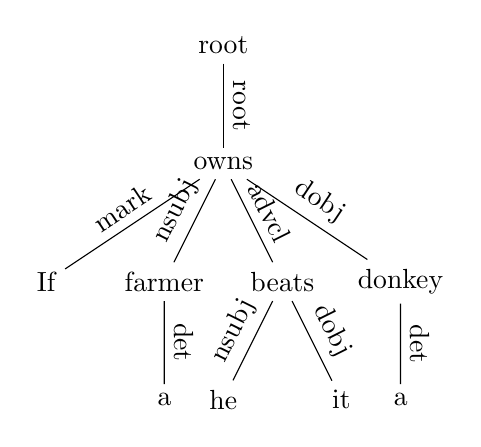
\begin{tikzpicture}[grow=down, sloped]
\node {root}
    child {
        node {owns}
        child {
            node {If}
            edge from parent
            node[above] {mark}
        }
        child {
            node {farmer}
            child {
                node {a}
                edge from parent
                node[above] {det}
            }
            edge from parent
            node[above] {nsubj}
        }
        child {
            node {beats}
            child {
                node {he}
                edge from parent
                node[above] {nsubj}
            }
            child {
                node {it}
                edge from parent
                node[above] {dobj}
            }
            edge from parent
            node[above] {advcl}
        }
        child {
            node {donkey}
            child {
                node {a}
                edge from parent
                node[above] {det}
            }
            edge from parent
            node[above] {dobj}
        }
        edge from parent
        node[above] {root}
    };
\end{tikzpicture}
\caption{M1} \label{fig:M1}
\end{figure}


\begin{equation}
NP < NN \$ VP
\end{equation}

An NP over an NN and w/ sister VP

\begin{equation}
NP < (NN < dog) \$ (VP <<\# (barks > VBZ))
\end{equation}

An NP both over an NN over `dog' and with
a sister VP headed by `barks' under VBZ

\subsection{Corefferences}
Corefferences (or anaphora) is essential in order to create advanced discourse, since it is what allows us maintain a topic beond the first mention. Without corefferences we couldn't even express simple logical statements such as transitivity: `a man's brother's brother is his brother' etc.

Identifying corefferences (or resolving anaphora) is hence an important part of converting natural language into logic. The issue is not touched upon in Visser's paper, which casually sidesteps the problem by assigning variables to all mentioned entities.

For the subtask of resolving simple pronouns a solution could be to work in terms of subjects, objects, indirect objects and so on. However if not earlier, this certainly fails for pronouns seperated from their antecedent by sentence bounderies. Also we want to resolve other kinds of corefferences, such as `John, the farmer, owns a donkey', where `the farmer' and `John' reffers to the same entity.

It quickly becomes clear that the problem is not only syntactical. In the sentence `John and his wife had a farm. He took care of the donkeys' we could substitute `He' with `She' and to change the refferant of the pronoun. In this case we need semantic knowledge of genders to proceed.

In my project I have taken advantage of the corefference tagger built into Stanford CoreNLP\cite{lee2013deterministic}\cite{lee2011stanford}\cite{raghunathan2010multi}. In the following section I will summerize the workings of this machine, made to work across large texts as well as simple sentences.

Correference tagging is one part of computational linguistics where machine learning algorithms still haven't been able to outperform large itterative applications of linguistic heuristics. Of course the procedure assumes (most likely) machine learned postagging and named entity recognization, but the main algorithm is transparent and deterministic.

The idea is to iteratively go over the text with different `sieves'. The below example explains each step with an example I have adopted from \cite{lee2013deterministic}:

\begin{quotation}
John is a farmer. He owned a stubborn donkey.
A girl was looking at the donkey.
``It was my favorite,'' John said to her.
\end{quotation}

\begin{description}
\item[Mention detection]
The first step is to identify all noun phrases (NP) and personal (PRP) and possesive (PRP\$) pronouns. This information is easily pulled from the postree. Notice we also identify nested mentions:

[John]$_1^1$ is [a farmer]$_2^2$. [He]$_3^3$ owned [a stubborn donkey]$_4^4$.\newline
[A girl]$_5^5$ was looking at [the donkey]$_6^6$.\newline
``[It]$_7^7$ was [[my]$_9^9$ favorite]$_8^8$,'' [John]$_{10}^{10}$ said to [her]$_{11}^{11}$.

All mentions are initially assigned to seperate entities (entity ids). The entities are also attached information we can easily pull from the postree, such as `a girl: {number: singular, gender: female}' which are used for the following rules.
\item[Speaker Sieve]
The purpose of this first sieve is to link self referring pronouns to speakers. Speakers are identified simply by their connection to verbs such as `say' and proximity to the quotations. In our case the pronoun `my' gets linked to `John':

[John]$_1^1$ is [a farmer]$_2^2$. [He]$_3^3$ owned [a stubborn donkey]$_4^4$.\newline
[A girl]$_5^5$ was looking at [the donkey]$_6^6$.\newline
``[It]$_7^7$ was [\textbf{[my]$_9^1$} favorite]$_8^8$,'' \textbf{[John]$_{10}^{9}$} said to [her]$_{11}^{11}$.

In conversational text we would store information about the speakers in our entities. Thus we could e.g. match mentions of `you' to the speaker of the previous quote we saw.

We also note restrictions for future use, so we don't risk corefferencing an `I' with a `he' etc.
\item[String Match]
The second step is to merge entities reffered to by exactly the same string. In our case we have two mentions of `John':

\textbf{[John]$_1^1$} is [a farmer]$_2^2$. [He]$_3^3$ owned [a stubborn donkey]$_4^4$.\newline
[A girl]$_5^5$ was looking at [the donkey]$_6^6$.\newline
``[It]$_7^7$ was [[my]$_9^1$ favorite]$_8^8$,'' \textbf{[John]$_{10}^{1}$} said to [her]$_{11}^{11}$.
\item[Relaxed String Match]
This third sieve doesn't get activated by our example. It will try to remove relative clauses and other text following the head word of a mention, and do an exact match of the result. For example [John] and [John, whose donkey loves him] will correctly be merged.

Like the `String Match' sieve, we are not doing anything fancy here, and we will incorrectly corefference the two mentions of `John' in: `[John, who loves donkeys] and [John, who hates donkeys] were brothers.'
\item[Precise Constructs]
The `Precise Constructs' sieve uses a lot of common patterns that link metions. In our case two `X is Y' patterns are found:

\textbf{[John]$_1^1$} is \textbf{[a farmer]$_2^1$}. [He]$_3^3$ owned [a stubborn donkey]$_4^4$.\newline
[A girl]$_5^5$ was looking at [the donkey]$_6^6$.\newline
``\textbf{[It]$_7^7$} was \textbf{[}[my]$_9^1$ \textbf{favorite]$_8^7$},'' [John]$_{10}^1$ said to [her]$_{11}^{11}$.

Other patterns include acronyms and appositives. For example [Canadian Donkey \& Mule Association] and [CDMA] are linked, because the second is tagged as an acronym and it matches the upper case letters of the first one. An appositive is usually a pattern `X, Y, ...' where Y is another description of X.
\item[Strict Head Match A, B, C] are simply rules strip mentions down to their head word and try to find exact matches. This is similar to `Relaxed String Match', but more radical. In our case we correctly get a link between `a stubborn donkey' and `the donkey':

[John]$_1^1$ is [a farmer]$_2^1$. [He]$_3^3$ owned \textbf{[a stubborn donkey]$_4^4$}.\newline
[A girl]$_5^5$ was looking at \textbf{[the donkey]$_6^4$}.\newline
``[It]$_7^7$ was [[my]$_9^1$ favorite]$_8^7$,'' [John]$_{10}^1$ said to [her]$_{11}^{11}$.

Linking mentions based on their head word is dangerous. e.g. `University of Oxford' and `University of Cambridge' both have `University' as their head word, but are (obviously?) different entities. To combat this a lot of strict rules must be observed. These are however gradually weakened in sieve B and C.
\item[Proper Head Noun Match] could be called `Strict Head Match D'. It is the weakest form of the sieve, as it has only the three contraints: two mentions of the same entity cannot have one included in the other, they cannot contain words reffering to conflicting geographical locations, and they cannot have different numbers. e.g. [donkeys] and [at least 5 donkeys].
\item[Pronoun Match]
This last sieve is perhaps the most important one. It is done in the end so that we may have as much data in our entities as possible for matching. Using guesses on gender, number and animacy we can make our final merges:

\textbf{[John]$_1^1$} is [a farmer]$_2^1$. \textbf{[He]$_3^1$} owned [a stubborn donkey]$_4^4$.\newline
\textbf{[A girl]$_5^5$} was looking at \textbf{[the donkey]$_6^4$}.\newline
``\textbf{[It]$_7^4$} was [[my]$_9^1$ favorite]$_8^4$,'' [John]$_{10}^1$ said to \textbf{[her]$_{11}^{5}$}.

As always there are a few contraints put on what can be merged. One rule is that the distance between pronun and antecedent must be maximum 3 sentences.
\end{description}

After the final step different post processing options are usually performed. For example singleton mentions are often discarded. That would mean we got rid of `a musician' and `my favorite'.

The reason the rules are applied in the order above is to give the most certain rules the highest priority.

The Stanford procedure above is currently the strongest competitor in various correference competitions.

\subsection{Semantics via dependencies}
This subsection's content...

\section{Implementation}
8pagish
This subsubsection's content...

There is not a big first order logic component in my project, but in the following it will often be useful to refer to the following structure

\begin{haskell}
data Prop =
    T | F
  | Not   Prop
  | And   Prop Prop
  | Or    Prop Prop
  | Predi Ref [Ref]
  | Exist Ref Prop
  | All Ref Prop
  | Impl Prop Prop
\end{haskell}

And since we are going to deal with some large computer generated formulas, I've implemented a simple simplification function, which simlply applies basic identities for $\top$ and $\bot$, and a comnbination of De Morgan's laws and the implication identity to eliminate negations.

One interesting part is that since the simplifyer has no look ahead, it will sometimes not find all applicable simplifications in one pass. For example
%
\begin{haskell}
simplify (Not (Impl p F)) = Not (simplify (Impl p F))
                          = Not (Not simplify p)
                          = Not (Not q)
\end{haskell}
%
Hence we need to run it a couple of times to get a good result. We can run it until the output doesn't change, or even simpler, just use a function like
%
\begin{haskell}
fexp :: (a -> a) -> Int -> (a -> a)
fexp f e = (iterate (f.) id) !! e
\end{haskell}

\subsection{My implementaiton of DPL semantics}

Syntactically we will be using the following structure

\begin{lstlisting}
data DPL =
    DT | DF
  | DComp DPL DPL
  | DOr DPL DPL
  | DNot DPL
  | DImpl DPL DPL
  | DExists Ref
  | DPredi Ref [Ref]
\end{lstlisting}

Below are some direct implementation of the semantics for DPL. We use the types
\begin{lstlisting}
type Assignment = [(Ref, Val)]
type Relation = Assignment -> [Assignment]
\end{lstlisting}
This differs from the indirect set of types are used in the earlier formalisms:
\begin{lstlisting}
type Assignment = [(Ref, Val)]
type Relation = Assignment -> Assignment -> Bool
\end{lstlisting}

intuitive

uses well known isomorphism

more direct

The later is very difficult to implement, since the semantics require quantification over all assignments. Like for composition.

\begin{lstlisting}
:: Relation
true = id
false = const []

predi1 :: [Val] -> Ref -> Rel
predi1 f k = filter (\as -> elem (get k as) f)

predi2 :: [(Val,Val)] -> Ref -> Ref -> Rel
predi2 f k l = filter (\as -> elem (get k as, get l as) f)

:: Relation -> Relation
neg r = filter (\as -> null (r [as]))

:: Relation -> Relation -> Relation
comp = flip (.)
impl s r = rnot (s `comp` (rnot r))
\end{lstlisting}
Then comes the most interesting one. To ``randomly reset'' a variable, we have to make sure that we have all assignments in the cross product of new values for the variable and what was there before.

Bum bum. Maybe we should just use a set, then we could overwrite variable assignments
\begin{lstlisting}
exist :: Ref -> [Val] -> Rel
exist k vs ass = [a : as | a <- news, as <- olds]
	where olds = map (filter ((/=k) . fst)) ass
	      news = [(k,v) | v <- vs]
\end{lstlisting}

\subsection{Handling variables}
One thing I haven't found much \cite{visser1999donkey}
Stanford: \cite{lee2013deterministic}
\cite{lee2011stanford}
\cite{raghunathan2010multi}
Coreferences
Using the parse tree and NPs

Something that's very interesting is when to use free variables and when to use bound variables. We can think of free variables as actors known by the context and bound variables as actors introduced in the sentence. So if we had `The farmer had a friend. His name was Anders', we could write the first part as $\exists y \cdot friends(x,y)$ and the second part as $name(y, `Anders')$. This is important to keep compositionality, but it does of course raise the interesting question of how to make sure that the variable for `Anders' in the first and the second sentence is the same.

In addition to being essential for composition, free variables are also very useful for information extraction type sentences. We can immagine writing a curious researcher writing into a search engine `farmers who like donkeys' which translates into $farmer(x) \cdot likes(x,y) \cdot \triangle \cdot \exists y \cdot donkey(y)$.

So how do we know when to include an $\exists$ and when not to?

The coreference parser does however not find entities that are only mentioned once. Hence to make the later processing simpler, we assign those entitie to free variable now as well.

The task is slightly complicated by the fact that NP's can be nested, so `The farmer and the donkey' is a NP consisting of two smaller NP's `The farmer' and `the donkey' seperated by `and'.

We resolve this by assigning top down, overwriting `word to ref' assignments with fresh variables as we go deeper down the tree. This way, for our short sentence, we might end up with the assignment $\{`The': `y', `farmer': `y', `and': `x', `the': `z', `donkey': `z'\}$

I parse the parse tree using parsec\cite{leijen2001parsec}

\begin{lstlisting}
toMapping :: [Ref] -> PosTree Word -> ([Ref], Map Int Ref)
toMapping vs (Leaf _ _) = (vs, empty)

toMapping vs tr@(Phrase "NP" subs) = (vs', submaps `union` np)
  where np = mapInterval 0 (tsize tr) v
        (v:vs', submaps) = toMapping vs (Phrase "" subs)

toMapping vs (Phrase _ []) = (vs, empty)
toMapping vs (Phrase _ (sub:subs)) = (vs'', p `union` shifted)
  where (vs', subm) = toMapping vs (Phrase "" subs)
        shifted = mapKeys (+tsize sub) subm
        (vs'', p) = toMapping vs' sub
\end{lstlisting}

where $tsize :: PosTree Word -> Int$ gives the number of words in the tree

\subsection{Using machine learning}
The $\bowtie$ and $\triangle$ notation makes logic look close enough to natural language that it starts looking tempting to use machine learning methods such as those used in translation to translate.

My main problem here is that such translation requires large ammounts of dualingo data. It was out of scope for my project to try create such.

\subsection{Handcoding}
This is not as bad as it sounds. It is similar to montague and what the stanfordparser does for dependencies.

\subsection{Examples}
Until now we've been very focused on the same one or two simple sentences. To provide a better test bench for our approach, it is interesting to follow some sentences through the different levels of our approach.

\begin{enumerate}
\item
Some description?
\begin{description}[style=multiline, leftmargin=10.25em]
  \item[Natural language] If a farmer who owns a donkey, he beats it 
  \item[Dependency Graph] ... eh
  \item[Monadic DPL] $\Bowtie \cdot \triangle \cdot \exists x \cdot farmer(x) \cdot \triangle \cdot owns(x,y) \cdot \triangle \cdot \exists y \cdot donkey(y) \cdot \triangle \cdot \Bowtie \cdot beats(x,y)$
  \item[DPL] $\exists x \cdot farmer(x) \cdot \exists y \cdot donkey(y) \cdot owns(x,y) \rightarrow beats(x,y)$
  \item[FOL] $\forall x ( farmer(x) \rightarrow \forall y ( donkey(y) \wedge owns(x,y) \rightarrow beats(x,y)))$
\end{description}

\item The second item
\item
`John wants to marry a Spanish girl'

This one is hard because it is an example of existential non commitment. I bet we'll fail it.
\end{enumerate}

Extract D Testing 
We have already seen some screen shots of the working program; however, we provide two stringent tests 
for our program to ensure it works as intended, along with a test rig to fully analyse the program. In both test 
programs, I will run through the whole series of options available to the user, and ensure its correctness. 
However, I will also demonstrate its ability to visualise code, and hopefully provide valuable insights whilst 
debugging. 
5.1 Simple Program -BFS and DFS using the Visitor Pattern
This test program begins by creating an underlying tree structure…
This kind of debugging is intuitive, and simple to do within this framework. If you have an intuitive 
understanding of what the underlying model in your program should look like, it is fairly straight forward to 
spot bugs like this in  small code samples. Assuming a larger program is in use, the user must delve a little 
deeper into the part of the graph which they suspect the bug to exist in. This is obviously heavily aided by the 
JDT debugger itself. However, this test still shows the usability of the code in a small program, and shows 
that the code can cope with the different types of back links and cross links that can occur in a memory 
graph.

\section{Perspectives/Conclusions}
2pagish

What I learned

‘a summary of your achievements; a critical appraisal, describing what worked well and what could be 
improved; a discussion of the lessons you have learnt from the project.’
In the ‘Conclusions’ you summarise your work and then stand back from the project and assess it as 
objectively as you can. This shows the examiners that you are capable of evaluating your own work 
according to the standards of the field. It is acceptable to mention areas that were not very satisfactory
because this shows that you have learnt from the experience of doing the project.
There are often three moves starting with a summary of your work, then giving an evaluation, highlighting
both its achievements and limitations and finally the possible future extensions of the work. The Evaluation 
move may also be carried out as part of the Summary. The Conclusion is the mirror image of the 
Introduction, in that it starts with the narrow concerns of the project and widens out to more general 
statements about further work.

Move 1: Summary 
Summarises the most important aspects of the project work.  

I have successfully developed a novel local type inference algorithm

Move 2: Evaluation
Indicates what the writer considers to be the most valuable aspects of the project and its limitations. Provides 
an assessment of how far the aims of the project have been achieved.

my algorithm is exponential: whereas Gagnon's algorithm is 
polynomial. But experiments of execution time against method length show a typically linear trend whereas 
Gagnon's show a cubic trend

Move 3: Future Work
Gives possible extensions of the project. These suggestions may follow from the limitations mentioned in the 
Evaluation move. 

The greatest scope for future work is extending the application of my algorithm from local type inference to 
global type inference.

Should I make my latex file literate haskell? %bhttp://www.haskell.org/haskellwiki/Literate_programming

\lstinputlisting[language=Haskell]{Main.hs}

\section*{Acknowledgements}
Thanks to Samson

This section's content...\cite{visser1999donkey}

the PCFG parser\cite{klein2003accurate}

Érica is still super hot. And she rocks at linguistics.\cite{lander2001initial}

\subsection{Checklist}
Things learned from courses


\bibliographystyle{plain}
\bibliography{refs}

\end{document}
